\documentclass{llncs}

%% Latex documents that need direct input
%  The subcaption package allows for subfloat figure within a single float.
%  This package substitutes the depregated subfigure and subfig packages 
%  allowing to have subfigures within figures, or subtables within table 
%  floats. Subfloats have their own caption, and an optional global 
%  caption. 
%  >> WARNING: some journal templates from Springer and IEETrans might not
%              be compatible with this package forcing to use the 
%              deprecated packages instead.
\usepackage{subcaption}
\usepackage{subfig}

%  The following command loads a graphics package to include images 
%  in the document. It may be necessary to specify a DVI driver option,
%  e.g., [dvips], but that may be inappropriate for some LaTeX 
%  installations. 
\usepackage[]{graphicx}

% In order to include files without having a clear page using \include*, 
% the newclude package is required
\usepackage{newclude}

\usepackage{array}

% Required for acronyms
% use \acresetall to reset the acroyms counter
\usepackage{acro}

% Managing TODOES and unfinished figures
\usepackage{todonotes}

% Package for nice table
\usepackage{booktabs}

% Mathematics extra symols and commands
\usepackage{amssymb, amsmath}
\usepackage{pifont,amsfonts} % import fonts for tick and x-mark
  % define the extra symbols
  \newcommand{\cmarkgLarge}{\text{\large \color{green!60!black!80}\ding{51}}}
  \newcommand{\cmarkrLarge}{\text{\large \color{red!60!black!80}\ding{51}}}
  \newcommand{\xmarkLarge}{\text{\large \color{red!60!black!80}\ding{55}}}
  \newcommand{\cmark}{\text{\color{green!60!black!80}\ding{51}}}
  \newcommand{\xmark}{\text{\color{red!60!black!80}\ding{55}}}

%% In order to draw some graphs
\usepackage{tikz,xifthen}
\usepackage{tikz-qtree}
\usetikzlibrary{decorations.pathmorphing} % noisy shapes
\usetikzlibrary{fit}                                            % fitting shapes to coordinates
\usetikzlibrary{backgrounds}                                    % drawing the background after the foreground
\usetikzlibrary{shapes,arrows,shadows}
\usetikzlibrary{calc,decorations.pathreplacing,decorations.markings,positioning}
\usetikzlibrary{snakes,decorations.text,shapes,patterns}
\usetikzlibrary{snakes}
\usetikzlibrary{decorations}
\usetikzlibrary{decorations.text}
\usetikzlibrary{decorations.markings}
\usetikzlibrary{shapes}
\usetikzlibrary{patterns}
\usepackage{pgfplots}

%%----- To generate stand onle tikz legends
% argument #1: any options
\newenvironment{customlegend}[1][]{%
    \begingroup
    % inits/clears the lists (which might be populated from previous
    % axes):
    \csname pgfplots@init@cleared@structures\endcsname
    \pgfplotsset{#1}%
}{%
    % draws the legend:
    \csname pgfplots@createlegend\endcsname
    \endgroup
}%
% makes \addlegendimage available (typically only available within an
% axis environment):
\def\addlegendimage{\csname pgfplots@addlegendimage\endcsname}
\pgfkeys{/pgfplots/number in legend/.style={%
        /pgfplots/legend image code/.code={%
            \node at (0.295,-0.0225){#1};
        },%
    },
}
%%---- end tikz legends


% Clever cross referencing. Using cleverref, instead of writting 
% figure~\ref{...} or equation~\ref{...}, only \cref{...} is required.
% The package interprates the references and introduces the figure, fig.,
% equation, eq., etc keywords. \Cref forces first letter capital. 
% >> WARNING: This package needs to be loaded after hyperref, math packages,
%             etc. if used.
%             Cleveref is recomended to load late
%\usepackage{hyperref}
\usepackage{cleveref}

% SI units
\usepackage{siunitx}
% Define the money way to write
\sisetup{
  group-four-digits = true,
  group-separator = {,}
}

% Nice package with citeauthor
%\usepackage{natbib}        % contains the latex packages
\title{Classification of \acs*{sdoct} volumes with \acs*{lbp}: application to \acs*{dme} detection}
\titlerunning{Optimization approach to BUS lesion segmentation}  % abbreviated title (for running head)
%                                     also used for the TOC unless
%                                     \toctitle is used
%
\author{
  Guillaume~Lema\^itre\thanks{Corresponding author: \email{guillaume.lemaitre@udg.edu}}\inst{1,2} 
  \and Mojdeh~Rastgoo\inst{1,2}
  \and Joan~Massich\inst{2}
  \and Shrinivasan~Sankar\inst{2}
  \and D\'esir\'e~Sidib\'e\inst{2}
  \and Fabrice~M\'eriaudeau\inst{2}
}
%
\authorrunning{Lema\^itre et al.} % abbreviated author list (for running head)
%
%
\institute{ViCOROB, Universitat de Girona, Campus Montilivi, Edifici P4, \\17071 Girona, Spain,
\and
LE2I UMR6306, CNRS, Arts et M\'etiers, Univ. Bourgogne Franche-Comt\'e, \\12 rue de la Fonderie, 71200 Le Creusot, France
}
%\addtocmark{Hamiltonian Mechanics} % additional mark in the TOC
             % contains the Title and Autor info
%%%%%%%%%%%%%%%%%%%%%%%%%%%%%%%%%%%%%%%%%%%%%%%%%%%%%%%%%%%%% 
%>>>> uncomment following for page numbers
% \pagestyle{plain}    
%>>>> uncomment following to start page numbering at 301 
%\setcounter{page}{301} 
      % contains package and variables init.
%% Acronym definition example using glossaries package
%% \usepackage{acro} is required
%% 
%% For a powerful usage of the acro package look at http://tex.stackexchange.com/questions/135975/how-to-define-an-acronym-by-using-other-acronym-and-print-the-abbreviations-toge

\DeclareAcronym{us}{
  short = US,
  long  = Ultra-Sound
}

\DeclareAcronym{cad}{
  short = CAD,
  long  = Computer Aided Diagnosis
}

\DeclareAcronym{dm}{
  short = DM,
  long  = Digital Mammography
}

\DeclareAcronym{gt}{
  short = GT,
  long  = Ground Truth
}

\DeclareAcronym{bus}{
%  short = B\acs*{us},
%  long  = Breast \acifused{us}{\acs*{us}}{\acl*{us}}
short = BUS,
long= Breast Ultra-Sound
}

\DeclareAcronym{ml}{
  short = ML,
  long  = Machine Learning
}

\DeclareAcronym{acm}{
  short = ACM,
  long  = Active Contour Model
}

\DeclareAcronym{crf}{
  short = CRFs,
  long  = Conditional Random Fields
}

\DeclareAcronym{mrf}{
  short = MRFs,
  long  = Markov Random Fields
}

\DeclareAcronym{cv}{
  short = CV,
  long  = Computer Vision
}
\DeclareAcronym{icm}{
  short = ICM,
  long  = Iterated Conditional Modes
}
\DeclareAcronym{sa}{
  short = SA,
  long  = Simulate Anealing
}
\DeclareAcronym{gc}{
  short = GC,
  long  = Graph-Cuts
}

\DeclareAcronym{aov}{
  short = AOV,
  long  = Area Overlap
}

\DeclareAcronym{birads}{
  short = BI-RADS,
  long  = Breast Imaging-Reporting and Data System
}

\DeclareAcronym{mad}{
  short = MAD,
  long  = Median Absolute Deviation
}

\DeclareAcronym{qc}{
  short = QC,
  long  = Quadratic-Chi
}

\DeclareAcronym{sift}{
  short = SIFT,
  long  = Self-Invariant Feature Transform
}

\DeclareAcronym{bof}{
  short = BoF,
  long  = Back-of-Features
}

\DeclareAcronym{acr}{
  short = ACR,
  long  = American College of Radiology
}

\DeclareAcronym{fa}{
  short = FA,
  long  = Fibro-Adenoma
}

\DeclareAcronym{dic}{
  short = DIC,
  long  = Ductal Inflating Carcinoma
}

\DeclareAcronym{ilc}{
  short = ILC,
  long  = Inflating Lobular Carcinoma
}

\DeclareAcronym{fpr}{
  short = FPR,
  long  = False Positive Ratio
}

\DeclareAcronym{fnr}{
  short = FNR,
  long  = False Negative Ratio
}

\DeclareAcronym{fp}{
  short = FP,
  long  = False Positive
}

\DeclareAcronym{rbf}{
  short = RBF,
  long  = Radial Basis Function
}

\DeclareAcronym{dr}{
  short = DR,
  long  = Diabetic Retinopathy
}

\DeclareAcronym{dme}{
  short = DME,
  long  = Diabetic Macula Edema
}

\DeclareAcronym{oct}{
  short = OCT,
  long  = Optical Coherence Tomography
}

\DeclareAcronym{sdoct}{
  short = SD-OCT,
  long  = Spectral Domain OCT
}

\DeclareAcronym{amd}{
  short = AMD,
  long = Age-related Macular Degeneration
}

\DeclareAcronym{hog}{
  short = HOG,
  long = Histogram of Oriented Gradients
}

\DeclareAcronym{svm}{
  short = SVM,
  long = Support Vector Machines
}

\DeclareAcronym{bow}{
  short = BoW,
  long = Bag-of-Words
}

\DeclareAcronym{rf}{
  short = RF,
  long = Random Forest
}

\DeclareAcronym{roc}{
  short = ROC,
  long = Receiver Operating Characteristic
}

\DeclareAcronym{auc}{
  short = AUC,
  long = Area Under the Curve
}

\DeclareAcronym{lbp}{
  short = LBP,
  long = Local Binary Patterns
}

\DeclareAcronym{pca}{
  short = PCA,
  long = Principal Component Analysis
}

\DeclareAcronym{nlm}{
  short = NL-mean,
  long = Non-Local Mean
}

\DeclareAcronym{lopo}{
  short = LOPO,
  long =  Leave-One-Patient Out
}

\DeclareAcronym{lbptop}{
  short = LBP-TOP,
  long =  Local Binary Pattern histogram from Three Orthogonal Planes
}

\DeclareAcronym{se}{
  short = SE,
  long =  Sensitivity
Planes
}

\DeclareAcronym{sp}{
  short = SP,
  long =  Specificity
Planes
}

\DeclareAcronym{sw}{
  short = SW,
  long =  sliding window 
Planes
}      % contains the acronims 

%% Select inputing only one part of the document
%\includeonly{content/intro/intro}   % the file wihtout .tex
%\includeonly{content/other/other_content}
 
\begin{document} 
\maketitle 

\begin{abstract}
This paper addresses the problem of automatic classification of \ac{sdoct} data for automatic identification of patients with \ac{dme} versus normal subjects.
Our method is based on \ac{lbp} features to describe the texture of \ac{oct} images and we compare different \ac{lbp} features extraction approaches to compute a single signature for the whole \ac{oct} volume.
Experimental results with two datasets of respectively 32 and 30 \ac{oct} volumes show that
regardless of using low or high level representations, features derived from \ac{lbp} texture have highly discriminative power.% for the task on hand.
 
Moreover, the experiments show that the proposed method achieves better classification performances than other recent published works.

\keywords{\acl{dme}, \acl{oct}, \acs{dme}, \acs{oct}, \ac{lbp}.}
\end{abstract}

%% Incldue the content without .tex extension
\acresetall  % reset the acronyms from the abstract
% include the figures path relative to the master file
\graphicspath{ {./content/intro/figures/} }

\section{Introduction}

Eye diseases such as \ac{dr} and \ac{dme} are the most common causes of irreversible vision loss in individuals with diabetes. It is estimated that eye diseases will cost US\$500 million annually in healthcare and associated costs in the United States alone~\cite{Sharma2005}. Moreover, the prevalence of DR is expected to grow exponentially and affect over 300 millions people worldwide by 2025~\cite{Wild2004}.
Early detection and treatment of \ac{dr} and \ac{dme} is the key to preventing blindness.
The detection and diagnosis of retinal diseases are based on the detection of vascular abnormalities or lesions in the retina. 
\Ac{cad} systems have focused on the automatic analysis of fundus images in past decades~\cite{Abramoff2010,Trucco2013}.
The use of fundus photography is limited to the detection of signs correlated with retinal thickening such as hard and soft exudates, hemorrhages or microaneurysms.
However, DME is characterized as an increase in retinal thickness within 1 disk diameter of the fovea center with or without hard exudates and sometimes associated with cysts~\cite{ETDRSG1985}.
Therefore, fundus photography cannot always identify the clinical signs of DME, for example cysts, which are not visible in the retinal surface. In addition, it does not provide any quantitative measurements of retina thickness or information about cross-sectional retinal morphology. 

Recently, optical coherence tomography (OCT) has been widely used as a valuable diagnosis tool for DME detection.
OCT is based on optical reflectivity and produces cross-sectional and three-dimensional images of the central retina, thus allowing quantitative retinal thickness and structure measurements. 

The new generation of OCT imaging, namely spectral domain OCT (SD-OCT) offers higher resolution and faster image acquisition over conventional time domain OCT. SD-OCT can produce 27,000 to 40,000 A-scans/seconds with an axial resolution of $3.5-6$ $\mu m$~\cite{Chen2005}. 

Many of the previous works on OCT image analysis have focused on the problem of retinal layers segmentation, which is a necessary step for retinal thickness measurements~\cite{Chiu2010,Kafieh2013}.
Few works have addressed the specific problem of DME and its associated features detection from OCT images. Quellec \textit{et al.}~\cite{Quellec2010} proposed a method for the identification of fluid-filled regions in SD-OCT images of the macula based on texture features extracted in the segmented retinal layers.
The authors in~\cite{Srinivasan2014} proposed a classification method for the detection of DME versus AMD and normal OCT images. The method is based on pre-processing to reduce the speckle noise in OCT images and flattening of the images to reduce the variation of retinal curvature among patients. Then, histograms of oriented gradients (HOG) are extracted in each image of a volume and a linear SVM is used for classification. On a dataset of 45 patients containing 15 normal subjects, 15 DME patients and 15 AMD patients, the methods achieved a correct classification of 100\%, 100\% and 86.67\% for AMD, DME and normal cases respectively. 
Venhuizen \textit{et al.}~\cite{Venhuizen2015} also proposed a method for OCT images classification using the bag of words (BoW) approach.
The method starts with the selection of interest points in each individual B-scan by keeping the points corresponding to the top 3\% vertical gradient values. Then, a $9\times 9$ patch of intensity values is extracted around each selected interest point, and PCA is applied to reduce the dimension of every patch from 81 ($9\times 9$) to 9. 
All extracted patches are used to create a codebook using k-means clustering, and the obtained codebook from training is used to represent each OCT volume as a patch occurrence histogram. Finally, this histogram is used as feature vector to train a Random forest (RF) with a maximum of 100 trees. The method was used to classify OCT volumes between AMD and normal cases and achieved an area under the ROC curve (AUC) of 0.984 with a dataset of 384 OCT volumes. 
The most similar work to ours is the work of Liu \textit{et al.}~\cite{Liu2011} who proposed a method for macular pathology detection in OCT images using local binary patterns (LBP) as features.
The method starts by aligning and flattening the images, then a 3-level multi-scale spatial pyramid is created and LBP histograms are extracted in each block at every level of the pyramid. All obtained LBP histograms are concatenated into a global descriptor whose dimension is reduced using PCA. Finally a SVM is used as classifier. The method achieved good results in detection OCT scan containing different pathology such as DME or AMD, with an AUC of 0.93 using a dataset of 326 OCT scans.  


In this paper, we propose a method for automatic identification of patients with DME versus normal subjects by classifying the OCT volumes. Our method is based on LBP features to describe the texture of OCT images and dictionary learning using the BoW approach~\cite{Sivic2003}.
However, we do not based on interest points selection as opposed to the work of 
Venhuizen \textit{et al.}~\cite{Venhuizen2015} who also employed the BoW approach. We rather divide the images into local patches and extract a dense set of LBP descriptors.
We also use the entire OCT volume and extract 3D-LBP features to describe the volume, which is different from the work of Liu \textit{et al.}~\cite{Liu2011} who classified only the foveal scan for each patient.
We will show in the experiments, Section 4, that using the 3D-LBP descriptor provides better classification performances than extraction LBP in each individual B-scan.

This paper is organized as follows. In Section~2, we describe the features extraction methodology and the classification approach based on the BoW method.
Section~3 shows experimental results using two different datasets and comparison with another approach. Finally, the paper ends with concluding remarks in Section~4.


%----------

%%% Local Variables:
%%% TeX-master: "../../master.tex"
%%% End:
          % the file wihtout .tex
% include the figures path relative to the master file
% \graphicspath{ {./content/method/figures/visual_cues/}{./content/method/figures/}}
\graphicspath{ {./content/method/figures/}}

\section{Materials and Methods}

 This section offers a general description of the methodology proposed for OCT volume classification, whereas further details of some elements involved in the methodology are found as subsections.
  
  The proposed method, as well as, its experimental set-up are outlined in Fig.\,\ref{fig:ML-scheme}.
  The methodology is formulated as a standard classification procedure.
  The available dataset with its acompaining \textcolor{red}{GT} are divided into training $(S1,l1)$ and testing $(S2,l2)$. 
  The final goal is to represent $S1$ and $S2$ in the feature space $F$ by supplying $(sxF,l1)$ as a training to a classifier, using the trained classifier to estimate $l2$ from $S2xF$ and comparing the estimation with the \textcolor{red}{GT}.
   To do so, the images forming the OCT volumes are preprocessed using non-local means (NL-means) algorithm \cite{buades2005non}. This algorithm preserve important details and textures of the original image, while reducing the noise.
   The mapping stage is used to determine a discrete set of elements (or structures) $Z$  which is used for representing the volume $s  in S$.
   The feature detection stage correspond to measurements done in $G(Z)$ used for representing $s$ in terms of $ZxG$. 
   This mapping and feature detection steps can be found as a single-steps in the literature.
   The feature extraction procedure combines the elements in $Z$ and its measurements $G(Z)$ to create the final feature space $F$ and project $s$ on it.
   
   The design choices are all illustrated in Fig.\,\ref{fig:ML-scheme} and discussed further in this section. The work here presented does not discuss in detail neither the mapping, nor the adopted classifier, further than this lines.
   As a possible mappings, for representing the volumes, 2D image slices of the volume and \color{red}{7x7x7}\color{black} sliding volumes, have been considered. 
   As a classifier, a \color{red}{Random Forest}\color{black} using 100 trees, has been considered.
   
\begin{figure}[h]
\centering{
  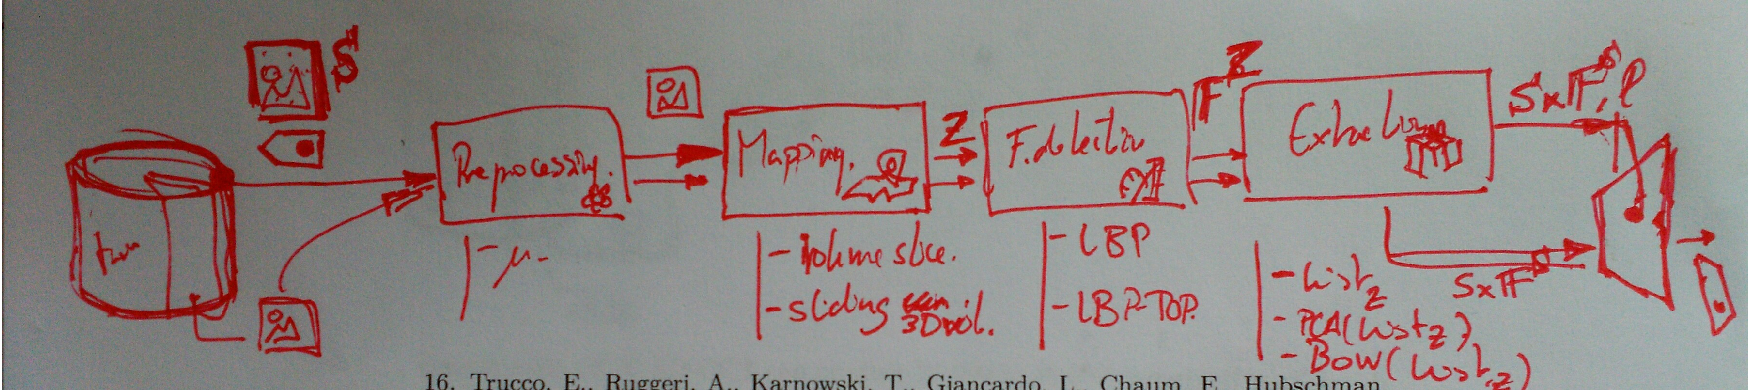
\includegraphics[width=1\textwidth]{mm.pdf}}
  \caption{Machine learning classification basic scheme}
  \label{fig:ML-scheme}
\end{figure}

\subsection{Data}
\color{red}{
\begin{itemize}
  \item cross-validation
  \item our dataset
  \item DUC dataset
\end{itemize}}\color{black}

For evaluation purposes, the results have been cross-validated, by splitting the data in training and testing using a \color{red}{loo}\color{black} strategy. In this manner for each round a pair \color{red}{dce,normal} has been selected to be used as the round test set, while the rest of the dataset has been used as a training. \color{red}{Doing the cross validation in this manner, has the limitation that despite the fact that the results are robust due to the cross validation, no results variance can be reported. However, and despite this limitation, LOO has been choose due to the reduced amount of OCT volumes available.}\color{black}

\color{red}{The dataset blablablabal...}\color{black}
\color{red}{The duc dataset blabla bla...}\color{black}

\subsection{Image pre-processing}
The pre-processing stage in the proposed methodology applies an image denoising method to reduce the speckle noise in OCT images. Since image details and texture of the original image are needed by the following stages in the method, non-local means (NL-means) algorithm \cite{buades2005non} is used. NL-means algorithm has the advantage to use all the possible self-predictions that the image can provide \cite{buades2005non} rather than local or frequency filters such as Gaussian, anisotropic or Wiener filters. \color{red}{Figure .. shows an OCT slice before and after denoising}\color{black}


\subsection{Features extraction}
Need to write something here !!!


\subsubsection{Low-level features} are extracted considering the whole volume using LBP and 3D-LBP descriptors. 
LBP is a discriminative rotation invariant feature descriptor proposed by Ojala et al. \cite{ojala2002multiresolution}. 
LBP descriptor encodes the intensity differences of a central pixel ($g_c$) with its neighboring pixels ($g_{p}$), within in a defined neighborhood of radius $R$. The differences are encoded in terms of binary patterns as in~Eq. \ref{Eq:LBP}: 

\begin{equation} \label{Eq:LBP}
LBP_{P,R} = \sum_{p=0}^{P-1}s(g_{p} - g_{c})2^{p},
\end{equation}
where $s(a) = 1$ if $a \geq 0$, and $s(a)=0$ otherwise. $P$ is the number of sampling points in the circle of radius $R$.

The binary patterns are calculated for each pixel in the given image and their histogram defines the final descriptor.
The LBP histograms are computed for each slice of the volume and are concatenated into a single histogram.


%In this research we consider rotation invariant features with uniform patterns. The uniform patterns are defined by the unifromity measure ($U$) of 2. Uniformity measure corresponds to the number of spatial transitions in the LBP pattern \cite{ojala2002multiresolution}. For instance patterns $00000000_{2}$ and $11111111_{2}$ have the U value of 0 while patterns like $01111111_{2}$ and $00000011_{2}$ have two transitions of 0/1 in their pattern, therfore they are considered as uniform patterns (see Eq. \ref{Eq:LBPru}). 
%\begin{equation}\label{Eq:LBPru}
%  LBP_{P,R}^{riu2} = 
%  \begin{cases}
%     \sum_{p=0}^{P-1}s(g_{p} - g_{c}) & \text{ if } U(LBP_{P,R}) \le 2\\
%       P+1 & \text{otherwise,}
%       \end{cases}
%    \end{equation}


The LBP features are extracted from each B-slice of the volume and their histograms are concatenated to build the first low-level descriptor. The second low-level descriptor is defined in a similar manner as the first one. However principal component analysis (PCA) is applied to the concatenated histograms in order to reduce the dimensions. The first and second low-level descriptors are obtained using the 2D LBP descriptor. However the third low-level feature is obtained using 3D-LBP (LBP-TOP). Zhao et al. \cite{zhao2007dynamic} proposed Local Binary Pattern histogram from Three Orthogonal Planes (LBP-TOP) as a dynamic texture descriptor. This descriptor is an extension to normal LBP while it considers texture descriptors along the temporal domain. LBP-TOP considers the LBP pattern in three orthogonal planes (see Fig. \ref{fig:LBPTOP-framework}), XY, XT and YT. The obtained LBP patterns from the three planes are concatenated to form the final descriptor. 

\begin{figure}
\centering{
  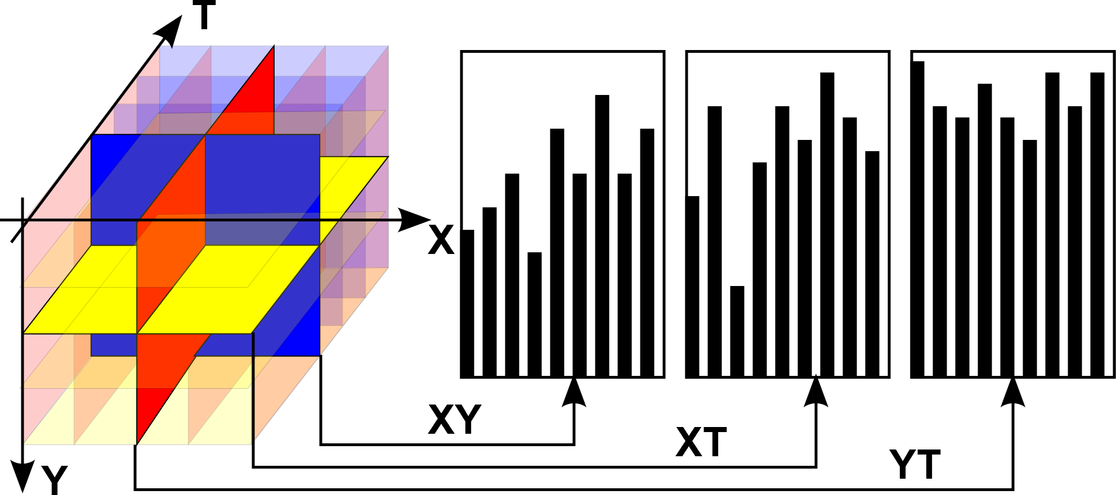
\includegraphics[width=0.40\textwidth]{LBPTOP_fig}}
\caption{LBP-TOP framework, the image is taken from \cite{JiangEtAl13}}
\label{fig:LBPTOP-framework}
\end{figure}



\subsubsection{High-level features} - are extracted using bag of features (BoF) approach which is illustrated in Fig. \ref{fig:BoF-framework}. After de-noising the images by non-local-mean approach, a patch detection step is carried out by identifying informative regions of the data. These patches can either be sampled densely or sparsely. The dense sampling extracts more information regarding the object appearance. However, it might retain redundant features. In the contrary sparse sampling is based on detecting salient key points from the most informative regions of the volume. Our proposed BoF approach is based on the first strategy. In this stage 2D-LBP (7$\times$7) and 3D-LBP-TOP patches (7$\times$7$\times$7) are extracted for each patient. Defining $N$ as the number of selected patches for each volume and $d$ as the number of feature dimensions, then each volume is characterized by a $N \times d$ feature matrix (see Fig. \ref{fig:BoF-framework}, ``feature extraction''). The next step in bag of features consists of building the dictionary of ``visual-words''. All the feature matrices of the training set are concatenated together and k-means clustering method (see Fig.\ref{fig:BoF-framework}, ``clustering'') is used to define the ``visual-words''. K-means is an iterative algorithm which finds k centroids by alternating assignment and update steps. The assignment steps is based on $L_{2}$ norm (Euclidean) distance. Different initialization methods can be used in order to assign the initial k clusters \cite {celebi2013comparative}, here the initial k clusters are selected based on greedy k-means++ method \cite{arthur2007k}. \textbf{Depending on the framework and application, different choices of the number of ``visual-words'' (number of $k$ clusters) can be made. In our framework, the number of clusters are varying in the range of [2 4 8 16 32 64 100]. SHOULD CHNAGE} Finally, the probability distribution (e.g., histogram) of the ``visual-words'' of each feature matrix is computed (feature quantization) and is used to feed the classifier to be trained. In the prediction stage, the histogram of the feature matrix corresponding to the new volume is computed using the previously learned dictionary and, finally, it is classified by the previously trained classifier.\\


% \tikzstyle{block} = [rectangle, draw, fill=gray!20, text = black,
    text width=6em, text centered, rounded corners, minimum height=4em , minimum width = 6em]
    % \tikzstyle{line} = [draw, -latex']
  \tikzstyle{myarrow}=[->, thick]
    \tikzstyle{line}=[-, thick]
    \tikzstyle{block2} = [rectangle, draw, fill=white!20,
    text width=6em, text centered, rounded corners, minimum height=4em, minimum width = 6em]
    \tikzstyle{block3} = [rectangle, draw, fill=gray!20, text = black,
    text width=7em, text centered, rounded corners, minimum height=4em , minimum width = 7em]
\def\blockdist{1}
\def\edgedist{1.5}
  %%%% The Framework Sparse Coding 

\begin{figure}
 \begin{center}
   \begin{tikzpicture}[node distance = 1cm,scale=0.6, every node/.style={scale=0.6}]
%(FEx.east|- FEx.south)
    \node [block2] (input) {Training image};
    %\node [block, right of = input, node distance = 2.8cm](Seg){Segmentation}; 
    \node [block, right of=input,node distance = 2.8cm](De){Denoising};
    \node [block, right of=De,node distance = 2.8cm](FEx){Feature extraction};
    \path (FEx.east)+(+0.8,0) node (g) {};
    
    %%% Sparse Coding Block
    \node [block3, right of=g,node distance = 1.7cm](DL){Dictionary learning /k-means};
    \node [block3, below of=DL,node distance = 2.5cm](PR){Projection};
    \begin{pgfonlayer}{background}
      \path (DL.west |- DL.north)+(-0.4,-0.1+\blockdist) node (a) {};
      \path (PR.east |- PR.south)+(+0.4,-0.7) node (b) {};          
      \path[fill=gray!10,rounded corners, draw=gray!20, dashed] (a) rectangle (b);
    \end{pgfonlayer}
\path (DL.west |- DL.north)+(+1.2,-0.5+\blockdist) node (SP) {\textbf{Bag of Features}};
\path (PR.east |- PR.south)+(-1.3,-0.4+\blockdist) node (c){};
\path (PR.east)+(-3.15,0) node (d) {};

%%% Testing 
\node [block, below of=FEx, node distance = 2.5cm](FE2){Feature extraction};
\node [block, below of=De, node distance = 2.5cm](De2){Denoising};
% \node [block, below of=Seg, node distance = 2.5cm](Seg2){Segmentation}; 
\node [block2, below of=input, node distance = 2.5cm](TestImg){Testing image};

%%% 
\node [block, right of=PR, node distance = 3.6cm](Pool){Visual words histogram};
\path (Pool.east) + (0.3,0) node (f){}; 
\path (Pool.east) + (0.2,-0.1) node (f1){}; 

%%% Classification
\node [block, right of = Pool, node distance = 3.5cm] (Pre){Prediction}; 
    \node [block, above of = Pre, node distance = 2.5cm] (Learn){Learning}; 
    \begin{pgfonlayer}{background}
      \path (Learn.west |- Learn.north)+(-0.4,-0.1+\blockdist) node (h) {};
    \path (Pre.east |- Pre.south)+(+0.4,-0.7) node (i) {};          
    \path[fill=gray!10,rounded corners, draw=gray!20, dashed] (h) rectangle (i);
\end{pgfonlayer}
\path (Learn.west |- Learn.north)+(+1.1,-0.5+\blockdist) node (Clas) {\textbf{Classification}};
\path (Pre.east |- Pre.south)+(-1.3,-0.4+\blockdist) node (j){};
\path (f1.north)+(0, 2.5) node (k) {};
\path (Pre.east) + (1.2,0) node (k1) {P(..)}; 

    % Draw edges
    \draw [line] (input) -- (De) -- (FEx); 
    \draw [myarrow] (FEx)-- (DL);
    \draw [myarrow] (DL) -- (PR) ; 
    \draw [line] (TestImg) -- (De2) -- (FE2); 
    \draw [myarrow] (FE2) -- (PR) ;
    \draw [line] (PR) -- (Pool); 
    \draw [myarrow] (Pool) -- (Pre); 
    \draw [line] (f1.north) -- + (0,2.5)(k.south); 
    \draw [myarrow] (k.south)+ (0,0.1)  -- (Learn.west); 
    \draw [myarrow] (Pre) -- (k1);

    \end{tikzpicture}
    \end{center}
    

\caption{Bag of features framework} 
\label{fig:BoF-framework}

\end{figure}

\subsection{Classification}

Random Forest is an ensemble of decision trees and was introduced by \cite{breiman2001random}.
The ensemble uses each tree to predict an output and finalize the ultimate
prediction by aggregating the outputs of all tress. This classifier learns the
data by training multiple decision trees on bootstrap samples of the original
data. Each bootstrap of D dimension is used for training one decision tree
and at each node, the best split among randomly (d << D) selected subset
of descriptors is chosen. Each tree is grown to its maximum length without
any pruning. In the prediction stage a sample is voted by each tree and it is
labeled by considering the majority of the votes.


%%% Local Variables: 
%%% mode: latex
%%% TeX-master: "../../master"
%%% End: 
 
% % include the figures path relative to the master file
% \graphicspath{ {./content/results/figures/} }

\section{Experiments and Validation }

\subsection{Datasets}

In this work, we validated our classification framework using two different datasets.

\begin{description}

\item[SERI]- datasets were acquired by Singapore Eye Research Institute (SERI), using CIRRUS TM (Carl Zeiss Meditec, Inc., Dublin, CA) \ac{sdoct} device. The datasets consist of 32 \ac{oct} volumes (16 \ac{dme} and 16 normal cases). Each volume contains 128 B-sane with  dimension of 512 $\times$ 1024 pixels.  All \ac{sdoct} images are read and assessed by trained graders and identifies as normal or \ac{dme} cases based on evaluation of retinal thickening, hard exudates, intraretinal cystoid space formation and subretinal fluid.

\item[Duke] - datasets published by Srinivasan et al. \cite{Srinivasan2014} were acquired in Institutional Review Board-approved protocols using Spectralis \ac{sdoct} (Heidelberg Engineering Inc., Heidelberg, Germany) imaging at Duke University, Harvard University and the University of Michigan. This datasets consist of 45 \ac{oct} volumes (15 \ac{amd}, 15 \ac{dme} and 15 normal). In this study we only consider a subset of the original data containing 15 \ac{dme} and 15 normal \ac{oct} volumes.

\end{description}

\begin{tiny}
  \begin{table}[Ht]
\caption{Obtained results using SERI datasets.}% using \ac{rf} with 100 trees. High-level features with \ac{bow} are obtained with $K$ = 32 visual-words.}
\centering
\begin{tabular}{lcclcclcccclcclcccclcclc}
\toprule
Features 	& & &\multicolumn{4}{c}{$8^{riu2}$}&	 & & & &\multicolumn{4}{c}{$16^{riu2}$}& & & & &\multicolumn{4}{c}{$24^{riu2}$} &\\
  \cmidrule(l){2-8}  \cmidrule(l){10-16}  \cmidrule(l){18-24}
	       & & & SE & & & SP & & & & & SE & & & SP & & & & & SE & & & SP & \\
\midrule
  	\ac{lbp}					& & & 43.75 & & & 43.75 & & & & & 37.50 & & & 50.00 & & & & & 50.00 & & & 62.50 & \\
 	\ac{lbptop}				& & & 56.25 & & & 62.50 & & & & & \textbf{87.50} & & & \textbf{75.00} & & & & & 68.75 & & & 68.75 & \\
	\ac{lbp}+\ac{pca}		& & & 50.00 & & & 62.50 & & & & & 56.25 & & & 37.50 & & & & & 68.75 & & & 68.75 & \\
	\ac{lbp}+\ac{bow}		& & & 50.00 & & & 81.25 & & & & & 57.50 & & & 68.75 & & & & & 50.00 & & & 50.00 & \\
	\ac{lbp}+\ac{bow}+\acs{sw}		& & & 75.00 & & & 87.50 & & & & & \textbf{81.25} & & & \textbf{75.00} & & & & & 68.75 & & & 62.5 & \\
	\ac{lbptop}+\ac{bow}+\acs{sw}		& & & 62.50 & & & 68.75 & & & & & 56.25 & & & 37.50 & & & & & 37.50 & & & 43.75 & \\
\bottomrule
\end{tabular}
\label{tab:SERI-data}
\end{table}
\end{tiny}

\subsection{Experiments \& results}

Both datasets are filtered to attenuate the effect of speckle noise.
SIRE dataset is processed using \ac{nlm} as stated in Sect.\,\ref{subsec:prepro}.
The different parameters were empirically tested and fixed such that the patch size, the search window and the filtering parameter were set to $(15 \times 15)$, $(35 \times 35)$ and $0.4$, respectively.
However, Duke dataset is already filtered using BM3D method~\cite{Srinivasan2014}.
For both datasets, \ac{lbp} and \ac{lbptop} features are extracted for different sampling points of 8, 16 and 24 for radius of 1, 2 and 3, respectively.
Two different mapping strategies are used: (i) the 2D B-scan for \ac{lbp} or the 3D volume for \ac{lbptop} and (ii) a set of 2D \ac{sw} of size $(7 \times 7)$ for \ac{lbp} or the 3D sub-volume for \ac{lbptop} of size $(7 \times 7 \times 7)$.
For the high-level representation, when \ac{pca} is applied, the eigenvectors associated with the largest $99\%$ cumulative eigenvalues are selected to reduce the number of dimensions. In \ac{bow} approach, an empirical search was performed to find the optimal number of visual words which is finally fixed to 32.
The number of trees for each \ac{rf} classifier was fixed to 100.
For evaluation purposes, all the results are expressed in terms of \ac{se} and \ac{sp} using a cross-validated \ac{lopo} strategy.
Thus, at each round a pair $(\ac{dme}, normal)$ is selected for testing while the rest acts as trainig.
Performing \ac{lopo} cross validation, has the limitation that despite acheaving robust results due to the cross validation, no variance in \ac{se} or \ac{sp}, can be reported.
A larger testing set can not be used here, due to the limited amount of available \ac{oct} volumes.

\begin{tiny}
  \begin{table}[Ht]
\caption{Obtained results using Duke datasets.}% using \ac{rf} with 100 trees. High-level features with \ac{bow} are obtained with $K$ = 32 visual-words.}
\centering
\begin{tabular}{lcclcclcccclcclcccclcclc}
\toprule
Features 	& & &\multicolumn{4}{c}{$8^{riu2}$}&	 & & & &\multicolumn{4}{c}{$16^{riu2}$}& & & & &\multicolumn{4}{c}{$24^{riu2}$} &\\
  \cmidrule(l){2-8}  \cmidrule(l){10-16}  \cmidrule(l){18-24}
	       & & & SE & & & SP & & & & & SE & & & SP & & & & & SE & & & SP & \\
\midrule
 	\ac{lbptop}				& & & 80.00& & & 93.33 & & & & & 73.33 & & & 86.67 & & & & & 73.33 & & & 86.67 & \\
	\ac{lbp}+\ac{bow}+\acs{sw}		& & & 80.00 & & & 86.67 & & & & & 86.67 & & & 100 & & & & &93.33 & & & 86.67 & \\
	\ac{lbptop}+\ac{bow}+\acs{sw}		& & & 80.00 & & & 86.67 & & & & & 86.67 & & & 86.67 & & & & & 60.00 & & & 80.00 & \\
\bottomrule
\end{tabular}
\label{tab:Duke-data}
\end{table}
\end{tiny}

\begin{description}

\item[Experiment \#1] is carried out on SERI dataset. Both low and high level feature representation are extracted and tested. The results are reported in Table~\ref{tab:SERI-data}.

\item[Experiment \#2] is carried out on the Duke dataset~\cite{Srinivasan2014}. The \ac{oct} volumes provided by this dataset are cropped, with different sizes.
Subsequently, the experiments involving the mapping using 2D B-scan do not comply with these requirements and thus are not carried out.
The obtained results for this experiment are shown in Table~\ref{tab:Duke-data}.

\item[Experiment \#3] presents a comparison of our best approaches with the method reported in~\cite{Venhuizen2015} in-house implemented and are expressed in Table~\ref{tab:ComparisonRefandOurs}.

\end{description}
% The SERI datasets are provided in complete \ac{oct} volumes by 512$\times$1024$\times$128 dimensions. Using this datasets, first the three low-level features such as \ac{lbp}, \ac{lbp}+\ac{pca} and \ac{lbptop} are extracted. The rotation invariant uniform ($riu2$) descriptors are calculated with the $P$ number of 8, 16 and 24 for the radius if 1, 2 and 3 respectively. The features are classified using RF with 100 tress. Table \ref{tab:LbPTopVolumeResult} shows the relative results for $8riu2$, $16riu2$, $24riu2$ and their combination $8riu2 + 16riu2 + 24riu2$. The results are presented in terms of \ac{se} and \ac{sp} percentages.

% The second experiment is carried out using high-level features and \ac{bow} approach, on SERI datasets. The first high-level feature \ac{lbp}+\ac{bow} is obtained by applying \ac{bow} with 32 visual-words on the previously low-level \ac{lbp} features (applied on each B-scan). The second and third high-level descriptors are obtained using a dense approach by applying the \ac{sw} of size (7$\times$7) on each B-scan and \ac{sw} of size (7$\times$7$\times$7) to the whole volume respectively. \ac{lbp}+\ac{bow}+\ac{sw} represent the second high-level feature where the 2D-\ac{lbp} features are extracted for each sliding window on each B-scan and the visual-words are selected from the pool, consisting of their histograms. The third high-level feature, \ac{lbptop}+\ac{bow}+\ac{sw}, is defined using \ac{lbptop}. By using the sliding window the 3D-\ac{lbp} features are extracted for each patch. Same as previous experiment with low-level features, the descriptors are calculated with the $P$ number of 8, 16 and 24 for the radius if 1, 2 and 3 respectively. The obtained results of this experiment are illustrated in Tab. \ref{tab:SERIBoWResult}.

% In order to compare our proposed framework the third experiment is carried out using the subsection of Duke datasets \cite{Srinivasan2014}. The OCT volumes provided by this datasets are of different volume size, cropped and denoised by the method of authors choice. Subsequently only the second experiment with high-level features and low-level \ac{lbptop} features comply with these requirements. The number of visual-words and the size of \ac{sw} for 2D and 3D features are the same than the previous experiment. The 2D and 3D \ac{lbp} features are extracted with $P$ number of 8, 16 and 24 for the radius if 1, 2 and 3 respectively. The obtained results for this experiment are shown in Tab. \ref{tab:DukeBoWResult}.
%----------

%%% Local Variables:
%%% mode: latex
%%% TeX-master: "../../master"
%%% End:

% % include the figures path relative to the master file
% \graphicspath{ {./content/results/figures/} }

\subsection{Results}


\begin{table}
\caption{Obtained results with Lbp, Lbp+pca and Lbp-Top features and RF with 100 trees on SERI dataset}
\centering
\begin{tabular}{lcclcclcccclcclcccclcclc}
\toprule
Features 	& & &\multicolumn{4}{c}{LBP}&	 & & & &\multicolumn{4}{c}{LBP+PCA}& & & & &\multicolumn{4}{c}{LBP-TOP} &\\
  \cmidrule(l){2-8}  \cmidrule(l){10-16}  \cmidrule(l){18-24}
	       & & & SE & & & SP & & & & & SE & & & SP & & & & & SE & & & SP & \\
\midrule
 $8^{riu2}$ 						& & & 43.75 & & & 43.75 & & & & & 50.00 & & & 68.75 & & & & & 56.25 & & & 62.50 & \\	
 $16^{riu2}$						& & & 37.50 & & & 50.00 & & & & & 68.75 & & & 56.25 & & & & & \textbf{87.50} & & & \textbf{75.00} & \\	
 $24^{riu2}$						& & & 50.00 & & & 62.50 & & & & & 56.25 & & & 37.50 & & & & & 68.75 & & & 68.75 & \\
 $\lbrace 8,16,24\rbrace^{riu2}$	& & & 37.50 & & & 56.25 & & & & & \textbf{68.75} & & & \textbf{68.75} & & & & & \textbf{81.25} & & & \textbf{81.25} & \\
\bottomrule
\end{tabular}
\label{tab:LbPTopVolumeResult}
\end{table}



\begin{table}
\caption{Obtained results for Lbp+BoW, LBP+BoW+SW, Lbp-Top+BoW+SW features and RF with 100 trees on SERI dataset. The BoW is computed with 32 visual words for all the experiments}
\centering
\begin{tabular}{lcclcclcccclcclcccclcclc}
\toprule
Features 	& & &\multicolumn{4}{c}{LBP+BoW}&	 & & & &\multicolumn{4}{c}{LBP+BoW+SW}& & & & &\multicolumn{4}{c}{LBP-TOP+BoW} &\\
  \cmidrule(l){2-8}  \cmidrule(l){10-16}  \cmidrule(l){18-24}
	       & & & SE & & & SP & & & & & SE & & & SP & & & & & SE & & & SP & \\
\midrule
 $8^{riu2}$ 						& & & 50.00 & & & 81.25 & & & & & 75.00 & & & 87.50 & & & & & 62.50 & & & 68.75 & \\	
 $16^{riu2}$						& & & 57.50 & & & 68.75 & & & & & 81.25 & & & 75.00 & & & & & 56.25 & & & 37.50 & \\	
 $24^{riu2}$						& & & 50.00 & & & 50.00 & & & & & 68.75 & & & 62.5 & & & & & - & & & - & \\
 %$\lbrace 8,16,24\rbrace^{riu2}$	& & & 37.50 & & & 56.25 & & & & & \textbf{68.75} & & & \textbf{68.75} & & & & & \textbf{81.25} & & & \textbf{81.25} & \\
\bottomrule
\end{tabular}
\label{tab:SERIBoWResult}
\end{table}


\begin{table}
\caption{Obtained results for LBP+BoW+SW, Lbp-Top+BoW+SW features and RF with 100 trees on Duke dataset. The BoW is computed with 32 visual words for all the experiments}
\centering
\begin{tabular}{lcclcclcccclcclc}
\toprule
Features 	& & &\multicolumn{4}{c}{LBP+BoW+SW}&	 & & & &\multicolumn{4}{c}{LBP-TOP+BoW} &\\
  \cmidrule(l){2-8}  \cmidrule(l){10-16}  
	       & & & SE & & & SP & & & & & SE & & & SP& \\
\midrule
 $8^{riu2}$ 						& & & 80.00 & & & 86.67 & & & & & 80.00 & & & 86.67 & \\	
 $16^{riu2}$						& & & 86.67 & & & 100.00 & & & & & 86.67 & & & 86.67 & \\	
 $24^{riu2}$						& & & 93.33 & & & 86.67 & & & & & 60.00 & & & 80.00 & \\
 %$\lbrace 8,16,24\rbrace^{riu2}$	& & & 37.50 & & & 56.25 & & & & & \textbf{68.75} & & & \textbf{68.75} & & & & & \textbf{81.25} & & & \textbf{81.25} & \\
\bottomrule
\end{tabular}
\label{tab:DukeBoWResult}
\end{table}


%----------

%%% Local Variables: 
%%% mode: latex
%%% TeX-master: "../../master"
%%% End: 


\section{Conclusions}
The work presented here addresses the automatic classification of \ac{sdoct} data to identify subjects with \ac{dme} versus normal.
Based on the reported results, the low level volume 3D features and high level 2D features using patches achieve the most desirable results in the experimental setup presented here.
The comparison against different datasets and methodologies, highlights that:
regardless of using low or high level representations, volume signatures derived from \ac{lbp} texture show high discriminative power for distinguishing \ac{dme} vs normal volumes.

%TOMORROW THE MOON !!


% Our method is based on \ac{lbp} features to describe the texture of \ac{oct} images and we compare different \ac{lbp} features extraction approaches to compute a single signature for the whole \ac{oct} volume.


\bibliography{./content/literature_review}   %>>>> bibliography data in report.bib
\bibliographystyle{splncs03}

\end{document} 
